\section{theory}\label{theory}

\subsection{Abstract Domains}\label{subsec:abstract_domains}

In the following sections we will describe the abstract domains of our value analysis.

\subsubsection{Abstract domain of strings as regular expressions}\label{subsubsec:abstract_domains_strings}

To represent the abstract domain of the family of SQL strings data types we have chosen regular expressions/languages.
Regular expressions/languages are chosen, as opposed to more powerful representations, for the decidable nature of inclusion and equality between them.

Let $REG$ denote the set of regular languages and
\begin{equation*}
    REG^{\leq n} = \{R \in REG \mid \forall w \in R : |w| \leq n\}.
\end{equation*}
In the following we do not distinguish between regular expressions and their languages.

In regards to abstract interpretation regulars expressions are not without their own quirks, as expressed in the following theorem.

The lattice of regular expressions $(REG, \subseteq, \cup, \cap)$ is not suited for abstract interpretation, as expressed by \autoref{thm:reg-lattice}.

\begin{restatable}{theorem}{reglattice}\label{thm:reg-lattice}
    $(REG, \subseteq, \cup, \cap)$ is a lattice, but not a complete one.
\end{restatable}

Thus we can not employ the Kleene fixed-point theorem to guarantee a fixed point and termination of our analysis.
We propose two solutions to overcome this limitation:
\begin{itemize}
    \item Limiting the size of the regulars expressions under consideration, this is sound in the case where the string data type which is abstracted over is fixed size;
    \item And to let the user define an abstract domain over the regular expressions that only contain finite elements.
\end{itemize}

To formalize the latter idea we introduce regular language partitions.

\begin{definition}
    Given a finite subset $REG^\subset \subset REG$ where $\bigcup REG^\subset = \Sigma^\star$.
    % todo Casper says: I am not sure if this restriction is useful.
    % and $\forall R_1, R_2 \in REG^\subset : R_1 \not\subset R_2 \land R_2 \not\subset R_1$.
    A regular language partition $p(REG^\subset)$ is a set where:
    \begin{itemize}
        % Casper says: I don't think the empty set in necessary.
        % \item $\emptyset \in p(REG^\subset)$,
        \item $\forall R \in REG^\subset : R \in p(REG^\subset)$,
        \item $\forall R_1, R_2 \in p(REG^\subset) : R_1 \cup R_2 \in p(REG^\subset)$,
        \item $\forall R_1, R_2 \in p(REG^\subset) : R_1 \cap R_2 \in p(REG^\subset)$.
    \end{itemize}
\end{definition}

% Tikzfigures
\begin{figure}
    \resizebox{7.5cm}{!}{
        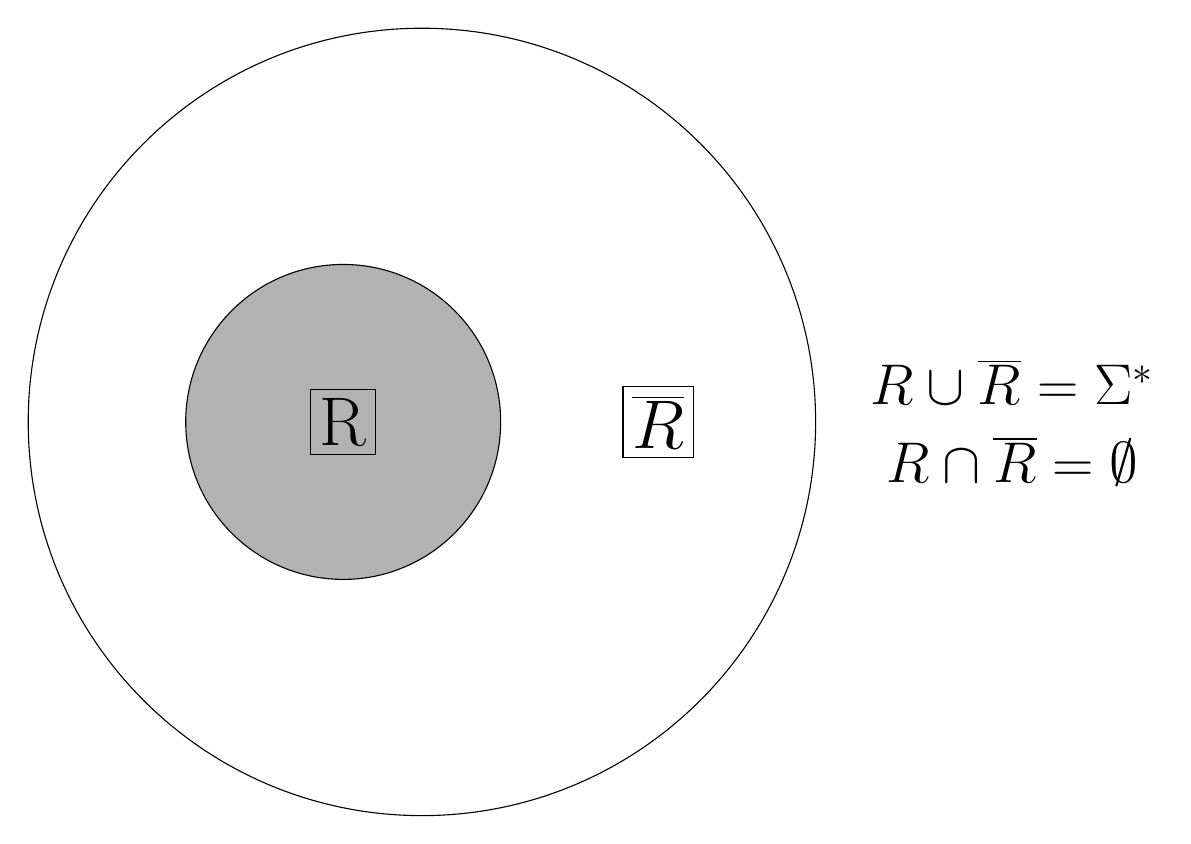
\begin{tikzpicture}
            \filldraw[fill=white, draw=black] (2,2) circle (5cm);
            \node [draw] at (5,2) {\Huge$\overline{R}$};
            \filldraw[fill=gray!60, draw=black] (1,2) circle (2cm);
            \node [draw] at (1,2) {\Huge R};
            \node at (9.5, 2.5) {\huge $R \cup \overline{R} = \Sigma^*$};
            \node at (9.5, 1.5) {\huge $R \cap \overline{R} = \emptyset$};
        \end{tikzpicture}
    }
    \caption{Regular language partition}
    \label{fig:tikz-reg-partition}
\end{figure}

\autoref{fig:tikz-reg-partition} illustrates a simple regular language partition. The regular language $R$ is represented by the gray circle and its complement $\overline{R}$ is represented by the white circle. The two circles together represent the entire regular language $\Sigma^*$ and their intersection is the empty set $\emptyset$.

\begin{figure}[!htb]
    \resizebox{6.5cm}{!}{
        \begin{tikzpicture}[scale = 0.5]
            \usetikzlibrary{calc}
            \node (a) [state] {\Huge$R \cup \overline{R} = \top = \Sigma^*$};
            \node (b1) [state, shift={($(a.south)+(3cm, -2.5cm)$)}] {\Huge $R$};
            \node (b2) [state, shift={($(a.south)+(-3cm, -2.5cm)$)}]{\Huge $\overline{R}$};
            \node (c) [state, shift= {($(a.south) + (0cm, -5.5cm)$)}] {\Huge $R \cap \overline{R} = \bot = \emptyset$};
            \draw (a) to (b1);
            \draw (a) to (b2);
            \draw (b1) to (c);
            \draw (b2) to (c);
        \end{tikzpicture}
    }
    \caption{Regular language partition as a lattice}
    \label{fig:tikz-reg-partition-lattice}
\end{figure}
\autoref{fig:tikz-reg-partition-lattice} illustrates the regular language partition as a lattice. The top element $\top$ is the entire regular language $\Sigma^*$ and the bottom element $\bot$ is the empty set $\emptyset$. The regular language $R$ and its complement $\overline{R}$ are the two elements in the partition.

\begin{theorem}\label{thm:finite-reg-lattice}
    $(REG^{\leq n}, \subseteq, \cup, \cap)$ is a complete lattice.
\end{theorem}

\begin{theorem}\label{thm:reg-partition-lattice}
    $(p(REG^\subset), \subseteq, \cup, \cap)$ is a complete lattice.
\end{theorem}


\subsubsection{Abstract domain of numbers as linear inequalities}\label{subsubsec:abstract_domains_numbers}

To represent the abstract domain of the family of SQL number data types when have chosen compound linear inequalities, more specifically compound linear inequalities which are algorithmically solvable by \gls{lp}.
\gls{lp} solvable compound linear inequalities where chosen for the prevalence of \gls{lp} solvers.
%todo
\todo{
    Casper says: We probably need a better reasons.
    Maybe look into NLP, MINLP, CP, SDP and convex optimization.
}

Let $LP^n$ be the set of solutions to \gls{lp} solvable compound linear inequalities where $\mathbf{x} \in X \in LP \implies \mathbf{x} \in \mathbb{R}^n$.\todo{
    Casper says: I feel like the description is more awkward than it needs to be.
}
And Let $ILP^n$ be the set integer solutions with the same constraint as above.
\autoref{thm:lp-lattice} demonstrates a similar problem as the one we encounter with the lattice $(REG, \subseteq, \cup, \cap)$.

\begin{theorem}\label{thm:lp-lattice}
    For $\mathcal{LP}^n \in \{ILP^n, LP^n\}$ : $(\mathcal{LP}^n, \subseteq, \cup, \cap)$ is a lattice, but not a complete one.
\end{theorem}

Again we employ a similar solution:

\begin{definition}
    Given a finite subset $LP_\subset^n \subset LP^n$ where $\bigcup LP_\subset^n = \mathbb{R}^n$.
    A \gls{lp} partition $p(LP_\subset^n)$ is a set where:
    \begin{itemize}
        \item $\forall X \in LP_\subset^n : X \in p(LP_\subset^n)$,
        \item $\forall X, Y \in p(LP_\subset^n) : X \cup Y \in p(LP_\subset^n)$,
        \item $\forall X, Y \in p(LP_\subset^n) : X \cap Y \in p(LP_\subset^n)$,
    \end{itemize}
\end{definition}

\begin{definition}
    Given a finite subset $ILP_\subset^n \subset LP^n$ where $\bigcup LP_\subset^n = \mathbb{Z}^n$.
    A I\gls{lp} partition $p(ILP_\subset^n)$ is a set where:
    \begin{itemize}
        \item $\forall X \in ILP_\subset^n : X \in p(ILP_\subset^n)$,
        \item $\forall X, Y \in p(ILP_\subset^n) : X \cup Y \in p(ILP_\subset^n)$,
        \item $\forall X, Y \in p(ILP_\subset^n) : X \cap Y \in p(ILP_\subset^n)$,
    \end{itemize}
\end{definition}

\begin{theorem}\label{thm:lp-partition-lattice}
    For $\mathcal{LP} \in \{ILP, LP\}$ : $(p(\mathcal{LP}_\subset^n), \subseteq, \cup, \cap)$ is a complete lattice.
\end{theorem}

\todo[inline]{
    Casper says: At this point it seems that the concept of a partition can be generalized.
}

\begin{definition}
    Given a finite subset $X \subseteq S$ of a lattice $S$ where $\bigsqcup X = \top$.
    A $S$-partition $p(X)$ is a set where:
    \begin{itemize}
        \item $\forall x \in X: x \in p(X)$,
        \item $\forall x, y \in p(X) : x \sqcup y \in p(X)$,
        \item $\forall x, y \in p(X) : x \sqcap y \in p(X)$,
    \end{itemize}
\end{definition}

\begin{theorem}
    For a non-complete lattice $S$ and a finite subset $X \subseteq S$ $(p(S)), \sqsubseteq, \sqcup, \sqcap)$ is a complete lattice.
\end{theorem}


% Let $A$ denote $m \times n$ matrix, $\mathbf{x}$ a $n \times 1$ column vector of variable and $\mathbf{b}$ a $m \times 1$ column vector of constants, then the solutions to the linear inequality $A \mathbf{x} \leq \mathbf{b}$ can be described as:
% \begin{equation*}
%     \{\mathbf{x} \in \mathbb{R}^n \mid A \mathbf{x} \leq \mathbf{b} \}
% \end{equation*}
% For the set of solutions of linear inequalities $A \mathbf{x} \leq \mathbf{b}$ and $A' \mathbf{x}' \leq \mathbf{b}'$ where $\mathbf{x}$ and $\mathbf{x}'$ are of the same size, their union and intersection are given by:
% \begin{align*}
%     \{\mathbf{x} \in \mathbb{R}^n \mid A \mathbf{x} \leq \mathbf{b} \}
%     &\cup
%     \{\mathbf{x} \in \mathbb{R}^n \mid A' \mathbf{x} \leq \mathbf{b'} \} \\
%     &=
%     \{
%         \mathbf{x} \in \mathbb{R}^n \mid A \mathbf{x} \leq \mathbf{b}
%                                     \lor A' \mathbf{x} \leq \mathbf{b}'
%     \}
% \end{align*}
% and
% \begin{align*}
%     \{\mathbf{x} \in \mathbb{R}^n \mid A \mathbf{x} \leq \mathbf{b} \}
%     &\cap
%     \{\mathbf{x} \in \mathbb{R}^n \mid A' \mathbf{x} \leq \mathbf{b'} \} \\
%     &=
%     \{\mathbf{x} \in \mathbb{R}^n \mid \begin{bmatrix} A \\ A' \end{bmatrix}  \mathbf{x} \leq \begin{bmatrix} \mathbf{b} \\ \mathbf{b}' \end{bmatrix} \}
% \end{align*}












